\documentclass[11pt]{article}
\usepackage{float}
\usepackage{amsfonts}
\usepackage[english,ukrainian]{babel}
    \title{\textbf{Применение Recurrent Sigmoid Piecewise нейрона для прогнозирования временных рядов}}
    \date{}
    
    \addtolength{\topmargin}{-3cm}
    \addtolength{\textheight}{3cm}
\usepackage{graphicx}
\begin{document}

\maketitle
\thispagestyle{empty}

\section*{Введение}
\section*{Постановка задачи}

Имеется временной ряд ${x_1, ..., x_N}$, сгенерированный некоторым вероятностным процессом $ \{X_t\} $ с неизвестными cовместными распределениями:
$$ p(x_{t+k}, x_{t}, x_{t-1}, ..., x_{t-n}). $$
Процесс $ \{X_t\} $ может быть как стационарным так и нестационарным. Если процесс нестационарный - в общем случае данная задача прогнозирования не имеет решения, так как вероятностные распределения нестационарного ряда в теории могут "меняться"\ как угодно, и распределения в будущем могут не иметь ничего общего с распределениями, на основе которых был сгенерирован имеющийся временной ряд. Однако на практике изменение вероятностных распределений нестационарных процессов с течением времени не происходит совершенно случайным образом. Поэтому прогнозирующие модели, оцененные на имеющемся в наличии временном ряде, обычно работают удовлетворительно на протяжении определенного периода времени даже при условии нестационарности соответствующего процесса.

Необходимо использовать данный временной ряд для нахождения прогнозирующей модели вида:
$$ \hat{x}_{t+k} = f^*(x_{t}, ..., x_{t-n}), $$
которая минимизирует математическое ожидание ошибки:
$$ f^* = argmin_f \{ E_{p(x_{t+k}, x_{t}, x_{t-1}, ..., x_{t-n})} [ L(f(x_{t}, ..., x_{t-n}), x_{t+k}) ] \}, $$
где $L: \mathbb{R} \times \mathbb{R} \to \mathbb{R}_{\geq 0} $ - функция ошибки. Часто используется либо квадратическая $ L(x, y) = (x-y)^2 $ либо абсолютная ошибка $ L(x, y) = |x-y| $. Поскольку рассчитать настоящее математическое ожидание невозможно (соответствующие вероятностные распределения неизвестны), вместо него используется среднее значение функции ошибки на тестовой подвыборке временного ряда:

$$ f^* = argmin_f \{ \frac{1}{M} \sum_{t=N-k-M+1}^{N - k}{L(f(x_t, ..., x_{t-n}), x_{t+k})} \} $$.

\section*{Основные существующие методы прогнозирования}
\textbf{Линейные модели на основе модели ARIMA}.
\\
Модель ARIMA(p,d,q) это модель для описания временного ряда $X_t$ следующего вида:
$$\Delta^dX_t = c + \sum_{i=1}^{p}{a_i\Delta^dX_{t-i}} + \sum_{j=1}^{q}{b_j\varepsilon_{t-j} + \varepsilon_t},$$
где:
\begin{itemize}
\item $\varepsilon_t$ - стационарный временной ряд, представляющий собой шум с нулевым математическим ожиданием;
\item $ c, a_1, ..., a_p, b_1, ..., b_q $ - параметры модели;
\item $\Delta^d$ - оператор разности временного ряда порядка d (последовательное взятие d раз разностей первого порядка — сначала от временного ряда, затем от полученных разностей первого порядка, затем от второго порядка и т. д.).
\end{itemize}
Существуют разные методы для построения прогнозирующих ARIMA моделей, 2 наиболее известных - это линейная регрессия и методология Бокса-Дженкинса. Линейная регрессия заключается в построении частного случая ARIMA модели вида:
$$X_t = \sum_{i=1}^{p}{a_iX_{t-i}} + a_0 ,$$
где вектор параметров $\vec{a} = [a_0, a_1, ..., a_p]$ оценивается с помощью метода наименьших квадратов:
$$ \vec{a} = {(A^TA)}^{-1}A^Tb ,$$
где $A, b$ - матрица и вектор получаемые из исходного временного ряда применяя скользящее окно размера $p$.
\\
Методология Бокса-Дженкинса позволяет оценивать полную ARIMA модель, но часто требует "экспертного вмешательства"\ для определения параметров $p,q,d$, так как существуют различные тесты для их определения, и необходимо выбирать тот либо иной тест и критические значения выбранного теста.
\\
\textbf{Искусственные нейронные сети}.
\\
Искусственные нейронные сети представляют собой систему взаимосвязанных искусственных нейронов, где каждый нейрон обычно реализует простую функцию вида:
$$ f(x;w) = u(w \cdot x); x,w \in \mathbb{R}^n $$
где $u: \mathbb{R} \to \mathbb{R} $ - некоторая нелинейная функция, называемая функцией активации. Наиболее популярные функции активации:
\begin{itemize}
\item $ReLU(x;w) = max(0,w \cdot x)$
\item $ \sigma(x;w) = \frac{1}{1 + e^{-w \cdot x}} $
\item $ tanh(x;w) = tanh(w \cdot x) = \frac{2}{1 + e^{-2 w \cdot x}} - 1$
\end{itemize}
В контексте задачи прогнозирования популярными являются искусственные нейронные сети прямого распространения (feedforward neural network) со структурой вида:
\begin{figure}[H]
\centering
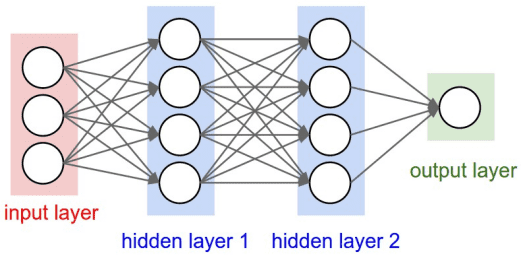
\includegraphics[scale=0.4]{/home/ivan/my_projects/nau_forecasting/docs/ff-neural-net.png}
\label{}
\end{figure}
которые по сути являются нелинейной вариацией AR-модели: $X_t = f(X_{t-1},...,X_{t-p})$ - где $f$ - функция, реализуемая нейронной сетью.
Настройка параметров нейронной сети, также называемая обучением, обычно производится применением некоторой вариации алгоритма градиентного спуска:
\begin{itemize}
\item Для относительно небольших сетей и временных рядов можно применять алгоритм Левенберга-Марквардта, который на практике часто находит значение параметров, близкое к оптимальному, и делает это значительно быстрее других алгоритмов (опять же, при условии небольшого количества параметров и длины временного ряда). 
\item Для больших сетей но относительно коротких временных рядов часто применяют "стандартный"\ алгоритм градиентного спуска либо его модификации типа алгоритма Adam, LBFGS, где градиент рассчитывается сразу для всего временного ряда.
\item Для больших сетей и длинных временных рядов используются "пакетные"\ вариации алгоритмов из предыдущего пункта, в которых на каждой итерации градиент рассчитывается только для определенного под-множества - "пакета"\ данных.
\end{itemize}
Кроме оптимизации непосредственно параметров нейронной сети с заданной структурой также необходимо определить саму структуру сети. Кроме варианта применения определенных эвристик для "ручного"\ задания структуры также возможно применение алгоритмов автоматического подбора структуры: наиболее популярными являются алгоритмы обучения с подкреплением, эволюционные алгоритмы и алгоритмы "семейства"\ МГУА. 
\\
\textbf{Рекуррентные нейронные сети}.
\\
В задачах обработки ествественного языка, таких как построение языковых моделей, автоматический перевод текста и пр. хорошо себя "зарекомендовали" рекуррентные нейронные сети на основе Long Short Term Memory (LSTM) и/или Gated Recurrent Unit (GRU) нейронов. Данные нейроны имеют схожую структуру, которая позволяет уменьшить влияние проблемы затухающего/взрывающегося градиента при обучении рекуррентных моделей с использованием Backpropagation Through time (BPTT) алгоритма на длинных последовательностях. За счет этого, на практике, сети с этими нейронами более стабильны в обучении и имеют большую "точность" при работе на длинных последовательностях. LSTM-нейрон имеет следующую структуру:
\\
\\
\begin{figure}[h]
\centering
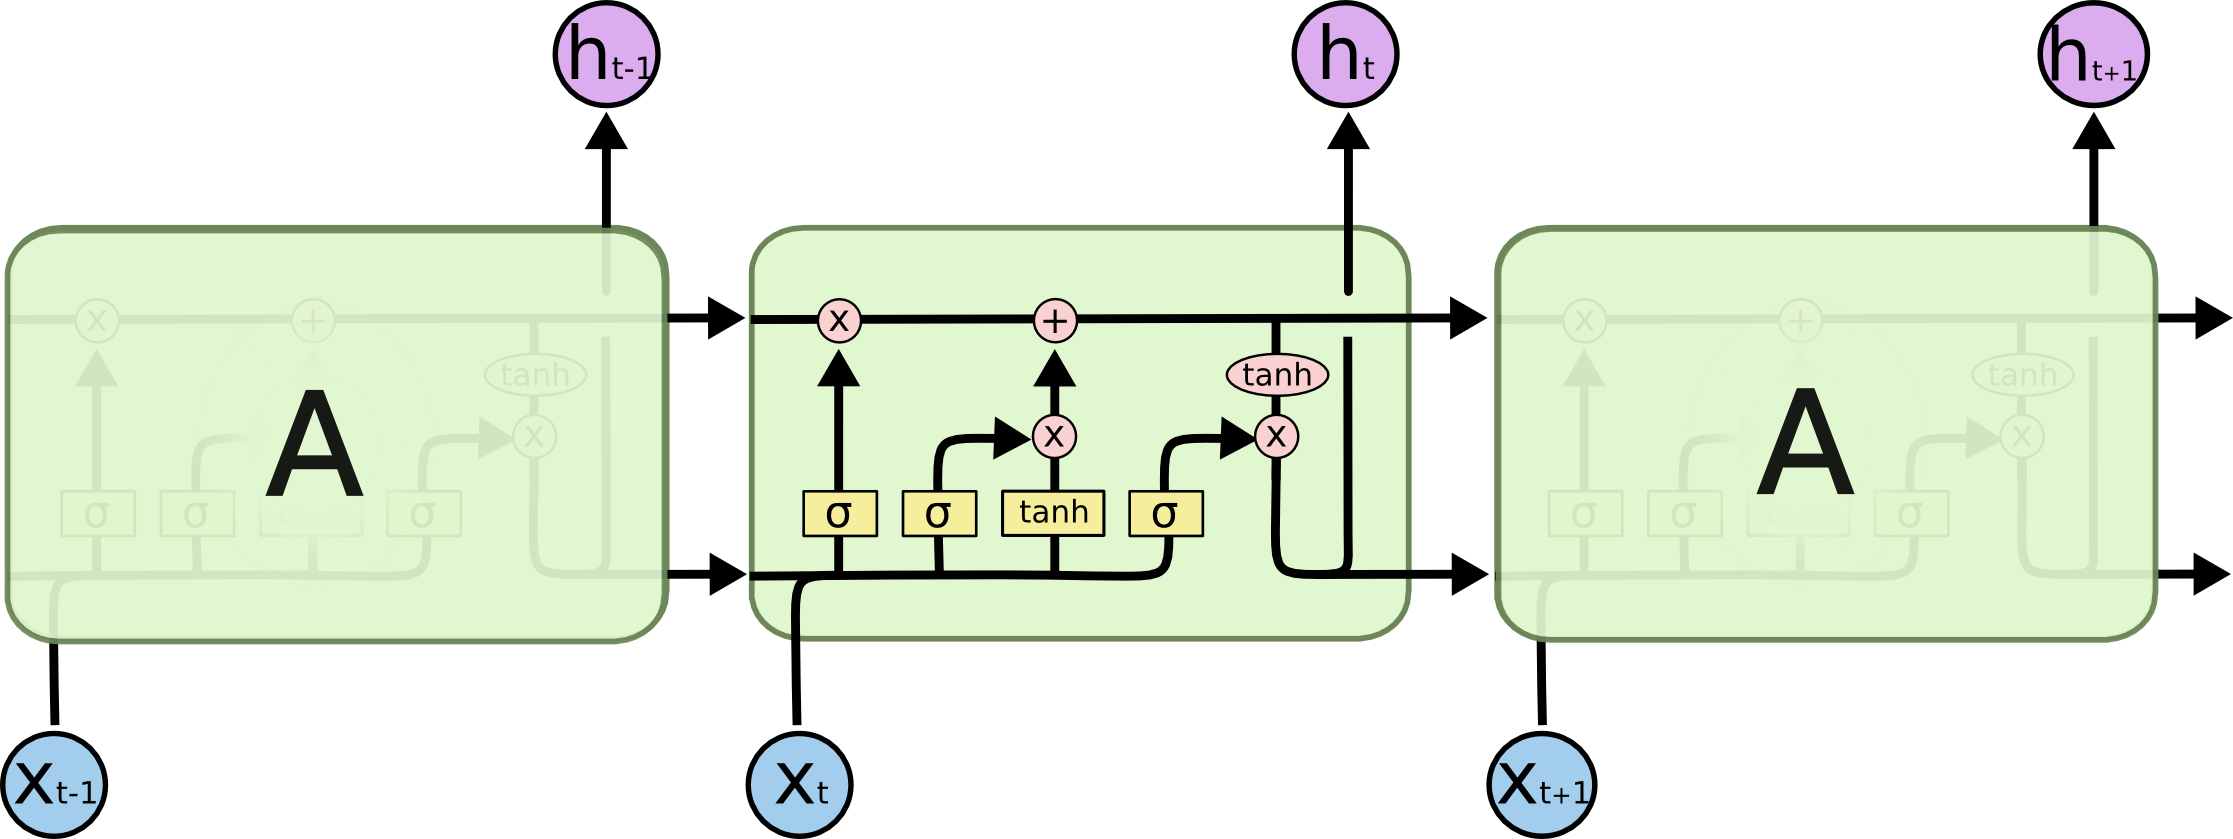
\includegraphics[scale=0.3]{/home/ivan/Downloads/LSTM3-chain.png}
\label{}
\end{figure}
\\
Полное математическое описание классического LSTM нейрона:
$$ f_t = \sigma( W_f \cdot [h_{t-1},x_t] + b_f) $$
$$ i_t = \sigma( W_i \cdot [h_{t-1},x_t] + b_i) $$
$$ \tilde{C_t} = tanh( W_C \cdot [h_{t-1},x_t] + b_C) $$
$$ C_t = f_t * C_{t-1} + i_t * \tilde{C_t} $$
$$ o_t = \sigma( W_o \cdot [h_{t-1},x_t] + b_o) $$
$$ h_t = o_t * tanh(c_t) $$
\\
\\
GRU нейрон это, по сути, упрощенная версия LSTM нейрона:
\begin{figure}[H]
\centering
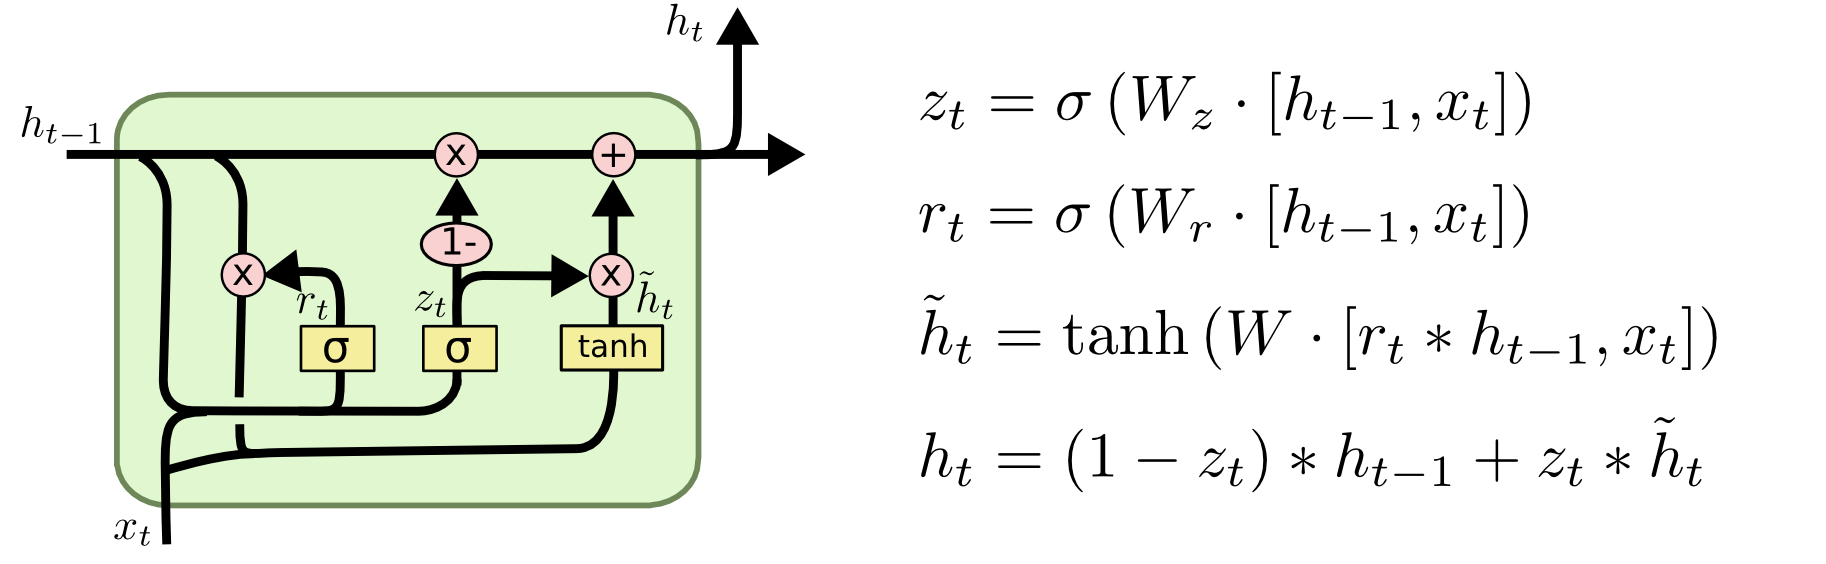
\includegraphics[scale=0.50]{/home/ivan/Downloads/LSTM3-var-GRU.png}
\label{}
\end{figure}
В данном нейроне вектор выходов $h_t$ так же "выполняет"\ роль вектора контекста, и используются следующие блоки:
\begin{itemize}
\item Блок обновления $z_t(x_t,h_{t-1};W_z)$, рассчитывающий веса в диапазоне $(0,1)$, которые применяются для рассчета нового вектора выходов (и, одновременно, контекста) $h_t$ исходя из вектора-кандидата $\tilde{h}_t$ и предыдущего вектора $h_{t-1}$
\item Блок "релевантности"\ $r_t(x_t,h_{t-1};W_r)$, рассчитывающий веса в диапазоне $(0,1)$, которые определяют "релевантность"/"важность"\ значений предыдущего выходного вектора $h_{t-1}$ при рассчете вектора-кандидата для нового выходного вектора $\tilde{h}_t$
\item Блок рассчета вектора-кандидата новых выходов $\tilde{h}_t(x_t,h_{t-1},r_t;W)$
\item Блок рассчета нового вектора выходов $h_t(h_{t-1},\tilde{h}_t,z_t)$ как взвешенной суммы соответствующих значений из предыдущего вектора $h_{t-1}$ и нового вектора-кандидата $\tilde{h}_t$, где веса для значений под индексом $i$ выбираются как $1-z_t[i]$ и $z_t[i]$ соответственно.
\end{itemize}
\textbf{Гибридные модели, boosting, bagging}.
\\
\textbf{ДОПОЛНИТЬ}

\section*{Recurrent Sigmoid Piecewise (RSP) нейрон}
В данной работе предлагается новая модель рекуррентного нейрона Recurrent Sigmoid Piecewise (RSP), в основе которой лежит Sigmoid Piecewise (SP) нейрон со следующей математической моделью:
$$ SP(x;w_+,w_-,s,k)=\frac{w_+ \cdot x}{1 + e^{-k(s \cdot x)}} + \frac{w_- \cdot x}{1 + e^{k(s \cdot x)}} $$
Используя обозначение сигмоидального нейрона:
$$\sigma(x;s)=\frac{1}{1+e^{s \cdot x}}$$
и $k=1$ получаем:
$$ SP(x;w_+,w_-,s)=\sigma(x;s)(w_+ \cdot x) + \sigma(x;-s)(w_- \cdot x) $$
Используя равенство $\sigma(x;-s)=1 - \sigma(x;s)$:
$$ SP(x;w_+,w_-,s) = (1 - \sigma(x;s))(w_- \cdot x) + \sigma(x;s)(w_+ \cdot x) $$
Если вместо одного SP нейрона описывается слой из N нейронов, то вместо векторов $w_+,w_-,s$ будут использоваться матрицы $W_+,W_-,S$:
$$ SP(x;W_+,W_-, S) = (1 - \sigma(x;S)) * (W_- \cdot x) + \sigma(x;S) * (W_+ \cdot x) $$
Введя обозначения $ z = \sigma(x;S) $, $a = W_- \cdot x$ и $b = W_+ \cdot x$ получаем:
$$ SP(x) = (1 - z) * a + z * b $$
Что очень похоже на блок рассчета нового вектора выходов в нейроне GRU:
$$ h_t = (1-z_t)*h_{t-1} + z_t*\tilde{h}_t $$
Таким образом, слегка изменив SP нейрон, можно получить его рекуррентную версию, Recurrent Sigmoid Piecewise (RSP) нейрон, который принимает на вход вектор $p_t=[h_{t-1}, x_t]$ и выдает $h_t$:
$$ h_t=RSP(p_t;W_+,W_-,S) = (1-\sigma(p_t;S))*(W_- \cdot p_t) + \sigma(p_t;S)*(W_+ \cdot p_t) $$
Либо же, по аналогии с LSTM/GRU нейронами, мат. модель RSP нейрона можно записать в несколько этапов/блоков:
$$ z_t = \sigma(S \cdot [h_{t-1}, x_t]) $$
$$ q_t = W_- \cdot [h_{t-1}, x_t] $$
$$ \tilde{h}_t = W_+ \cdot [h_{t-1}, x_t] $$
$$ h_t = (1 - z_t) * q_t + z_t * \tilde{h}_t $$
\\
И представить их в виде структурной схемы:
\\
\begin{figure}[H]
\centering
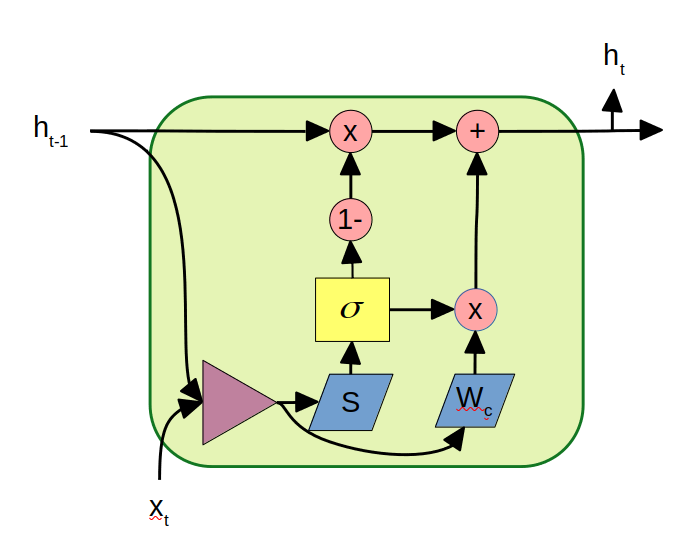
\includegraphics[scale=0.3]{/home/ivan/Documents/recurrent_sigmoid_piecewise_neuron_structure.png}
\label{}
\end{figure}

Поверхностно сравнив RSP нейрон с LSTM и GRU нейронами можно сделать следующие наблюдения:
\begin{itemize}
\item Математическая модель RSP нейрона проще (используется лишь один нелинейный сигмоидальный блок) чем модели LSTM и GRU нейронов. В задаче прогнозирования временных рядов более простые модели часто предпочтительны на практике.
\item При этом, RSP так же как и LSTM и GRU нейроны позволяет забывать определенные значения в векторе контекста при необходимости.
 
\end{itemize}
  


\section*{Применение рекуррентных сетей на основе RSP нейронов для прогнозирования временных рядов}
Стандартную линейную ARMA модель можно обобщить следующим образом:
$$ X_t = \varepsilon_t + f(X_{t-1}, ..., X_{t-p}) + g(\varepsilon_{t-1},...,\varepsilon_{t-q}) ,$$
где $f: \mathbb{R}^p \to \mathbb{R}, g: \mathbb{R}^q \to \mathbb{R} $ - некоторые функции, в общем случае нелинейные. Наиболее общее описание нелинейной ARMA модели будет иметь вид:
$$ X_t = \varepsilon_t + f(X_{t-1}, ..., X_{t-p}, \varepsilon_{t-1}, ..., \varepsilon_{t-q}) ,$$
где $f: \mathbb{R}^{p+q} \to \mathbb{R}$ - нелинейная функция. На основе этого обобщения предлагается следующая схема прогнозирования временных рядов:
\begin{figure}[H]
\centering
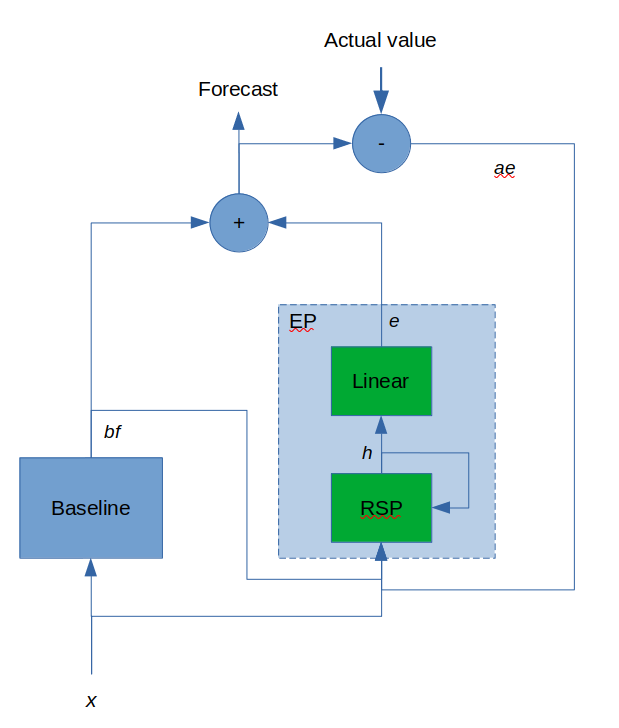
\includegraphics[scale=0.3]{/home/ivan/my_projects/nau_forecasting/docs/rsp_forecasting_scheme.png}
\label{}
\end{figure}
где:
\begin{itemize}
\item $x$ - входной вектор, предыдущие значения часового ряда (либо нескольких рядов)
\item \textbf{Baseline} - "базисная"\ прогнозирующая модель, рассчитывающая начальную оценку прогноза, например линейная регрессия; соответственно $b_t$ - базисное значение прогноза в момент времени $t$
\item \textbf{EP} - error prediction блок, рассчитывающий оценку ошибки прогноза $\hat{e}_t$ базисного метода на основе: входного вектора, самого значения базисного прогноза и настоящей ошибки прогноза с предыдущего шага
\item Базисный прогноз $b_t$ и оценка ошибки $\hat{e}_t$ складываются для получения финального прогноза: $f_t = b_t - \hat{e}_t$
\item На следующем шаге прогнозирования $t+1$ также рассчитывается настоящая ошибка прогноза с предыдущего шага $e_{t+1} = f_{t+1} - x_{t+1}$ и передается в блок рассчета ошибки прогноза текущего шага
\item Блок рассчета ошибки состоит из RSP нейрона и простого линейного слоя. По своей математической модели RSP нейрон может "естественным" способом рассчитывать новое значение коррекции как взвешенную сумму предыдущей ошибки и нового значения контекста.
\end{itemize}

Основным отличием данной прогнозирующей схемы от обычного использования прогнозирующей модели является блок предсказания ошибки. По сути, данный блок является нелинейной вариацией MA блока в модели ARMA. Использование этого блока позволяет схеме динамически реагировать на изменения в качестве прогноза базисной модели. Например, пускай для некоторого момента времени $t'$ получена достаточно большая ошибка прогноза $ e_{t'+1} = f_{t'+1} - x_{t'+1}, e_{t'+1} > 0 $, то есть прогноз модели оказался значительно больше реального значения. Одной из возможных причин может быть неожиданный для модели скачок "вниз" временного ряда:
\begin{figure}[H]
\centering
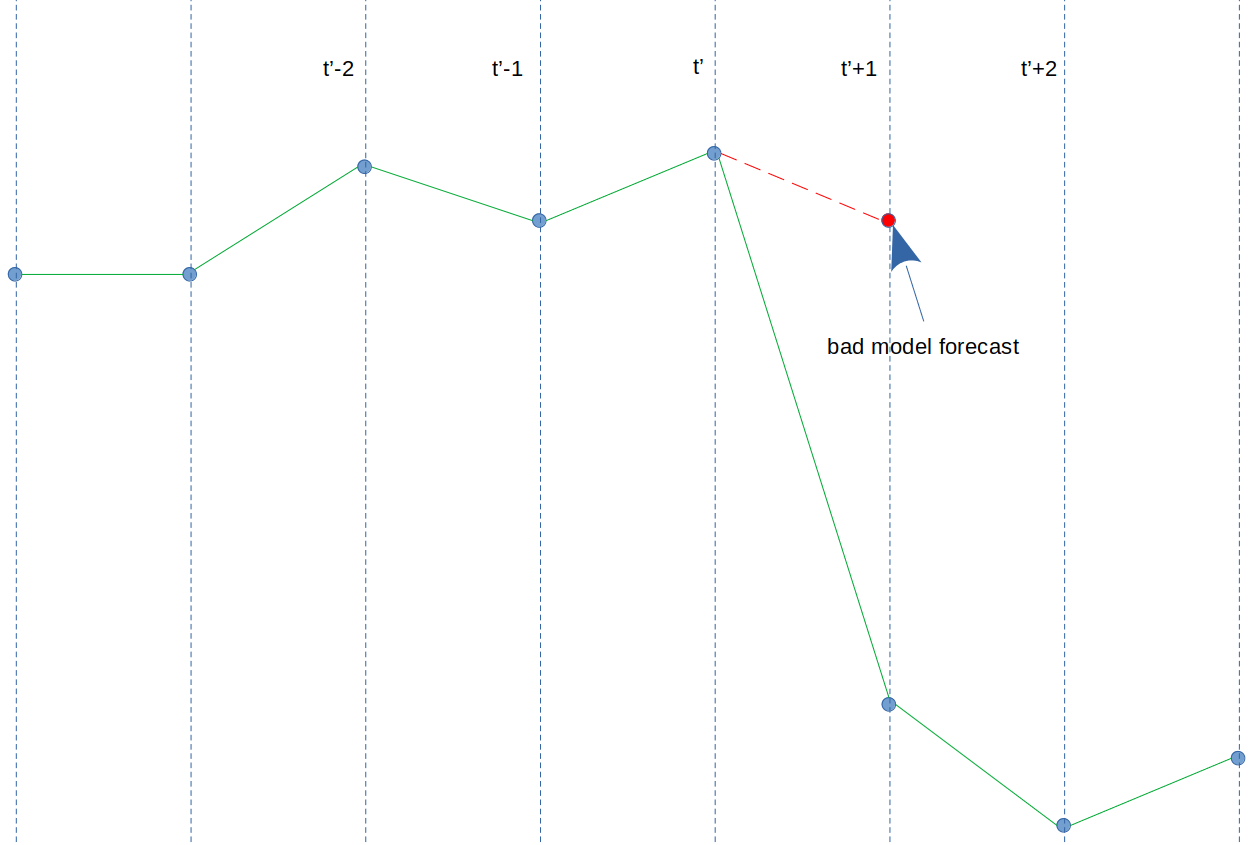
\includegraphics[scale=0.25]{/home/ivan/my_projects/nau_forecasting/docs/bad_model_forecast_too_high_example1_for_dynamic_EC_block.png}
\label{}
\end{figure}

В таком случае можно ожидать, что в момент времени $t'+1$ прогноз базисной модели также окажется больше, и блок ПО сможет его скорректировать путем предсказания оценки ошибки $ \hat{e}_{t'+2} > 0$. И наоборот - при неожиданном скачке "вверх" на шаге $t'$ будет получена большая негативная ошибка прогноза $ e_{t'+1} < 0 $ - тогда на шаге $t'+1$ прогноз базисной модели может также быть меньше реального значения, и блок ПО сможет его скорректировать путем предсказания оценки ошибки $\hat{e}_{t'+2} < 0$.
\\ 
Преимущества данной схемы:
\begin{itemize}
\item В качестве базисной модели можно брать прогнозирующую модель, полученную в результате применения любого существующего метода прогнозирования, и таким образом в процессе обучения EP блок будет пытаться только улучшать прогноз базисной модели.
\item Рассчет настоящего значения ошибки прогноза с предыдущего шага (шагов) в теории дает возможность EP блоку динамически "реагировать" на изменения в качестве прогноза.
\item Мат. модель RSP нейрона естественным образом подходит для рассчета некоторой ошибки прогноза.
\item В теории возможно поэтапное обучение EP и базисного блоков - на первом этапе обучаем параметры EP блока, на втором - фиксируем их и обучаем параметры базисного блока и т.д.
\end{itemize}

\section*{Практические примеры использования рекуррентных RSP сетей}
Для тестирования использовались показатели сердечного ритма 4 разных пациентов в разных состояниях:
\begin{figure}[H]
\centering
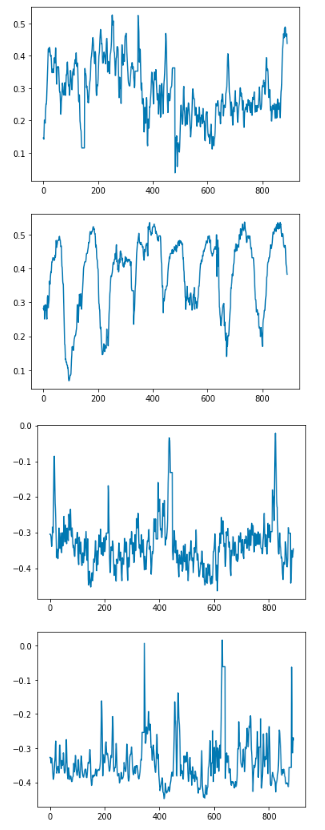
\includegraphics[scale=0.5]{/home/ivan/my_projects/nau_forecasting/docs/heart_rates_data.png}
\label{}
\end{figure}

Построив "базисную" модель - оптимальный линейный предиктор получаем следующие среднеквадратические ошибки прогноза на обучающей и тестовой выборке (усредненный по всем 4 пациентам):

$$ L^{baseline}_{train} = 0.0004731 $$
$$ L^{baseline}_{test} = 0.00048 $$

Пример прогнозов линейного предиктора для одного пациента на обучающей:
\begin{figure}[H]
\centering
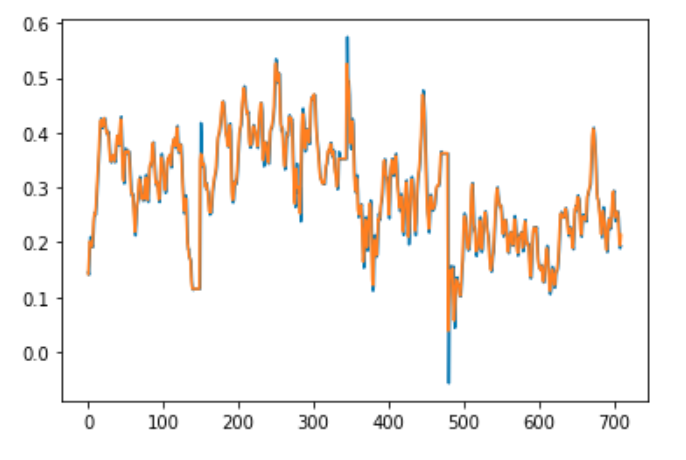
\includegraphics[scale=0.35]{/home/ivan/my_projects/nau_forecasting/docs/baseline_train_forecast.png}
\label{}
\end{figure}
 и тестовой:
\begin{figure}[H]
\centering
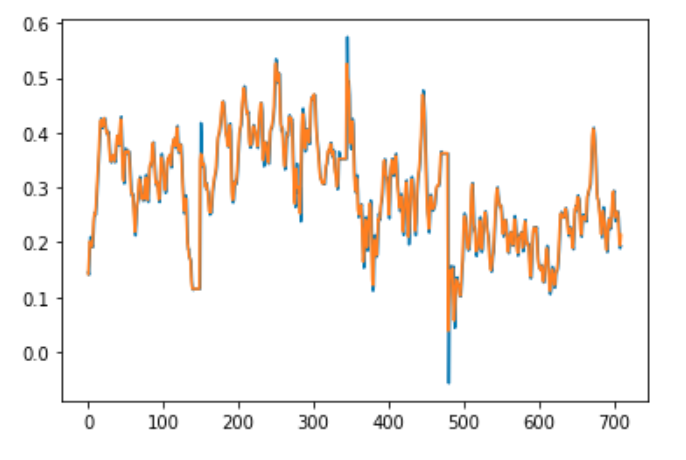
\includegraphics[scale=0.35]{/home/ivan/my_projects/nau_forecasting/docs/baseline_train_forecast.png}
\label{}
\end{figure}
выборках.

После "фиксации" базисного предиктора, добавления блока корекции на основе RSP нейрона и обучения его параметров получаем следующие значения среднеквадратических ошибок:
$$ L^{new}_{train} = 0.0004442 $$
$$ L^{new}_{test} = 0.00046 $$ 
что соотвествует приблизительно 5\% уменьшению среднеквадратической ошибки прогноза. 


\textbf{РАСШИРИТЬ ЭТУ ЧАСТЬ}

\section*{Выводы и дальнейшие направления работы}

\end{document}

